\section{Method}
\label{sec:method}

\subsection{Data}
\label{sec:data}

This study focuses on stellar rotation in the original \kepler\ field.
This is partly because \kepler\ provides the largest sample of published,
homogeneously measured rotation periods, and partly because its low Galactic
latitude allows us to marginalize over missing RV measurements and approximate
vertical velocity, \vz.

We combined two large rotation period catalogs constructed from original
\kepler\ data, from \citet{mcquillan2014} and \citet{santos2019}.
These two studies used different techniques to measure rotation periods from
\kepler\ light curves: autocorrelation functions and wavelets respectively.
The \citet{santos2019} study was specifically focused on cooler stars: K and M
dwarfs, and includes a larger number of rotation periods for these stars.
The combined catalogs provide a total of over 38,000 rotation periods.

\begin{itemize}
    \item{Describe cuts and Gaia crossmatch.}
    \item{Reddening calculation.}
    \item{Photometric temperatures.}
    \item{Binary and subgiant cuts?}
    \item{Gyro age cuts?}
    \item{Radial velocity replacement.}
    \item{Velocity calculation.}
\end{itemize}

To calculate kinematic ages, an estimate of vertical velocity, \vz, is
required.
The ideal way to calculated \vz\, and similarly, \vx\ and \vy, is to use 6D
positional and velocity information.
Many stars in the \kepler\ field do not have RV measurements and an
alternative approach must be taken to infer their vertical velocities (see
section \ref{sec:velocity_inference}).
However, a large number of \kepler\ rotators, over 10,000 of 34,000 {\it do}
have RV measurements from \gaia\ DR2 and \lamost.
Figure \ref{fig:existing_rvs} shows rotation period vs effective temperature
for all stars in the \mct\ and \citet{santos2019} catalogs, plotted in grey.
Stars with RV measurements are colored by their vertical velocity dispersion
(see section \ref{sec:velocity_dispersion} to see how we calculated velocity
dispersion).
\racomment{Discuss what this plot shows}.

Although RVs are available for a significant number of \kepler\ rotators
(almost one in three), few stars cooler than 4000 K have RV measurements.
This is due to the faint limits of the \gaia\ DR2 and \lamost\ surveys
(although RV measurements for fainter targets will be available in \gaia\
DR3).
Given that magneto-rotational evolution is poorly understood for M dwarfs, the
cool stars with missing RVs are arguably the ones we care most about.
For this reason, we attempted to compensate for the lack of RV measurements by
inferring vertical velocities for stars without RVs, to fill in the
low-temperature region of figure \ref{fig:existing_rvs} in section
\ref{sec:velocity_inference}.
\begin{figure}[ht!]
\caption{
Vertical velocity dispersion as a function of rotation period and effective
    temperature for \kepler\ stars with measured rotation periods.
Colored points show stars with RV measurements from \gaia\ or \lamost, with
    their color indicating their velocity dispersion.
Faint grey points show the combined \mct\ and \citet{santos2019} samples,
    including stars without RV measurements.
The coolest stars in this sample do not have RVs because they are faint.
}
  \centering 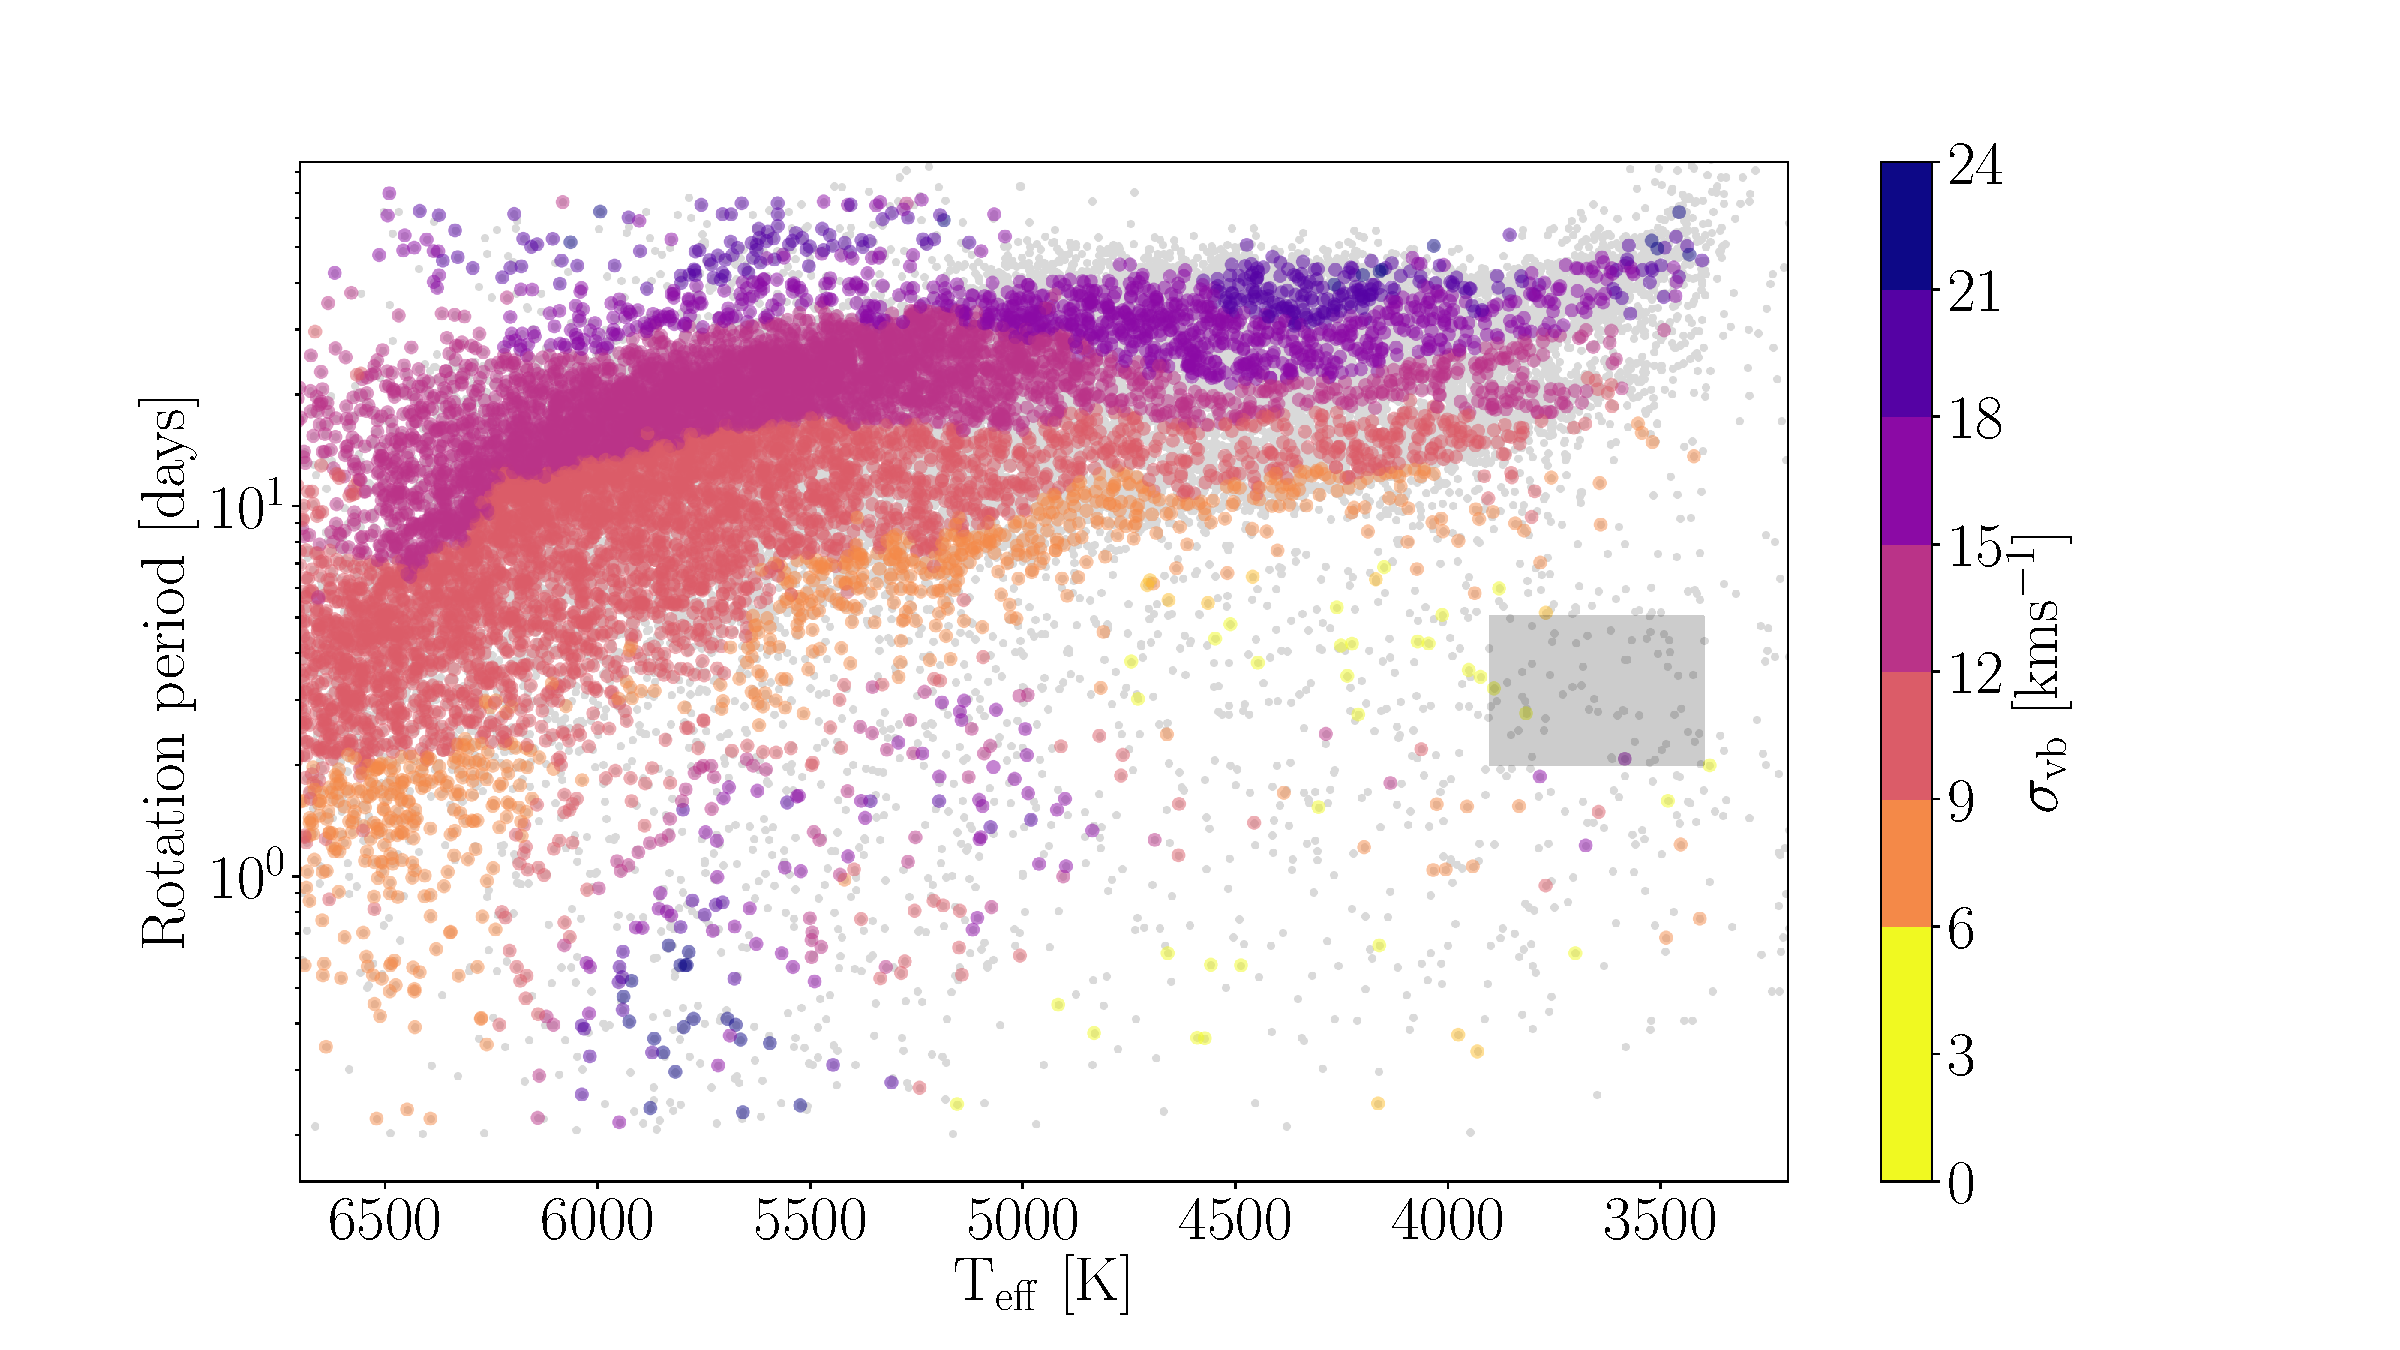
\includegraphics[width=1\textwidth]{existing_rvs}
\label{fig:existing_rvs}
\end{figure}


\subsection{Inferring 3D velocities (marginalizing over missing RV
measurements)}
\label{sec:velocity_inference}

It has been demonstrated that the dispersion in vertical velocity, \vz\, for a
group of stars increases with the age of that group (citations).
However, velocities in Galactocentric coordinates, \vx, \vy\ and \vz, can only
be calculated with full 6-D position and velocity information, \ie\ proper
motions, position and radial velocity.
In Angus \etal\ (2020) we showed that kinematic ages can be used to explore
rotational evolution and showed, in the appendix of that paper, that velocity,
\vb\ in the Galactic frame, which can be calculated without an RV measurement,
can be used as an approximation to \vz\ for \kepler\ stars.
This is because the \kepler\ field of view lies at relatively low Galactic
latitudes, ($\sim 5-20$\degrees), so the $z$-direction is similar to the
$b$-direction for \kepler\ stars.
However, \vb\ is only a close approximation to \vz\ at extremely {\it low}
latitudes, and even in the \kepler\ field, kinematic ages calculated with \vb\
instead of \vz\ are systematically larger because of extra noise introduced by
the imperfect translation between \vb\ and \vz .
In this work, we {\it infer} \vz\ by marginalizing over missing RV
measurements.

% Three-dimensional velocities in galactocentric coordinates: \vx, \vy, and \vz\
% can only be directly computed via a transformation from 3D velocities in
% another coordinate system, like the equatorial coordinates provided by \gaia:
% \mura, \mudec, and RV.
% For stars with no measured RV in \gaia\ DR2, \vx, vy, and \vz\ can still be
% inferred from positions and proper motions alone, by marginalizing over
% missing RV measurements.
For each star in our sample, we inferred \vx, \vy, and \vz\ from the 3D
positions and 2D proper motions provided in the \gaia\ DR2 catalog
\citep{brown2011}.
We also simultaneously inferred distance, (instead of using inverse-parallax),
to model velocities \citep[see \eg][]{bailer-jones2015, bailer-jones2018}.

Using Bayes rule, the posterior probability of the parameters given the data
can be written:
\begin{equation}
p(v_{\bf xyz}, D | \mu_{\alpha}, \mu_{\delta}, \alpha, \delta, \pi) =
    p(\mu_{\alpha}, \mu_{\delta}, \alpha, \delta, \pi | v_{\bf xyz}, D)
    p(v_{\bf xyz}) p(D),
\end{equation}
where D is distance, $\alpha$ is Right Ascension (RA), $\delta$ is declination
(dec), $\pi$ is parallax, $\mu_\alpha$ is proper motion in RA, and
$\mu_\delta$ is proper motion in dec.
For each star in the \kepler\ field, we explored the posteriors of these four
parameters using the {\it PyMC3} Hamiltonion Monte Carlo (HMC) sampler
\racomment{(citations)}.

We used the mean and covariance of the distance and velocity distributions of
\kepler\ targets {\it with} RV measurements to determine the 4D multivariate
Gaussian prior over $\log$(distance) and velocities.
3D velocities were calculated for every star with an RV measurement from
either \gaia\ or \lamost.
These velocities were then sigma-clipped at the 3-sigma level in all three
dimensions to remove large velocity outliers which may be caused by proper
motion or RV measurements with large errors.
We then calculated the mean and covariance of the multivariate Gaussian
distribution of \vx, \vy, \vz, and $\ln$(Distance).
We used this mean and covariance to construct our multivariate Gaussian prior.

We paid careful attention to the choice of prior.
Our goal was to infer the velocities of stars without RV measurements using a
prior calculated from stars {\it with} RV measurements.
However, stars with and without RVs are likely to be slightly different
populations, the parameters of which depend on the \gaia\ and \lamost\
selection function.
\racomment{Discuss selection functions.}
In particular, stars without RV measurements are more likely to be faint, and
therefore, less massive.
Lower-mass stars are, on average, older, and have larger velocity dispersions.
So a prior based on the velocity distributions of stars with RVs will not
necessarily reflect the velocities of those without.

For this reason, we tested how the choice of prior affected the velocities we
inferred.
We tested two priors: one calculated from the velocity distributions of the
brightest half of the RV sample (\gaia\ $G$-band apparent magnitude $<$ 13.9),
and one from the faintest half ($G > $ 13.9).
We selected the 500 faintest stars from the \gaia-\lamost\ RV sample to test
these two priors on.
We chose the faintest stars as these are the most likely to be similar to the
non-RV sample, and to enlarge the difference between the bright prior and the
test sample.
The results of this test are shown in figure \ref{fig:prior_test}

\begin{figure}[ht!]
\caption{
    }
  \centering
    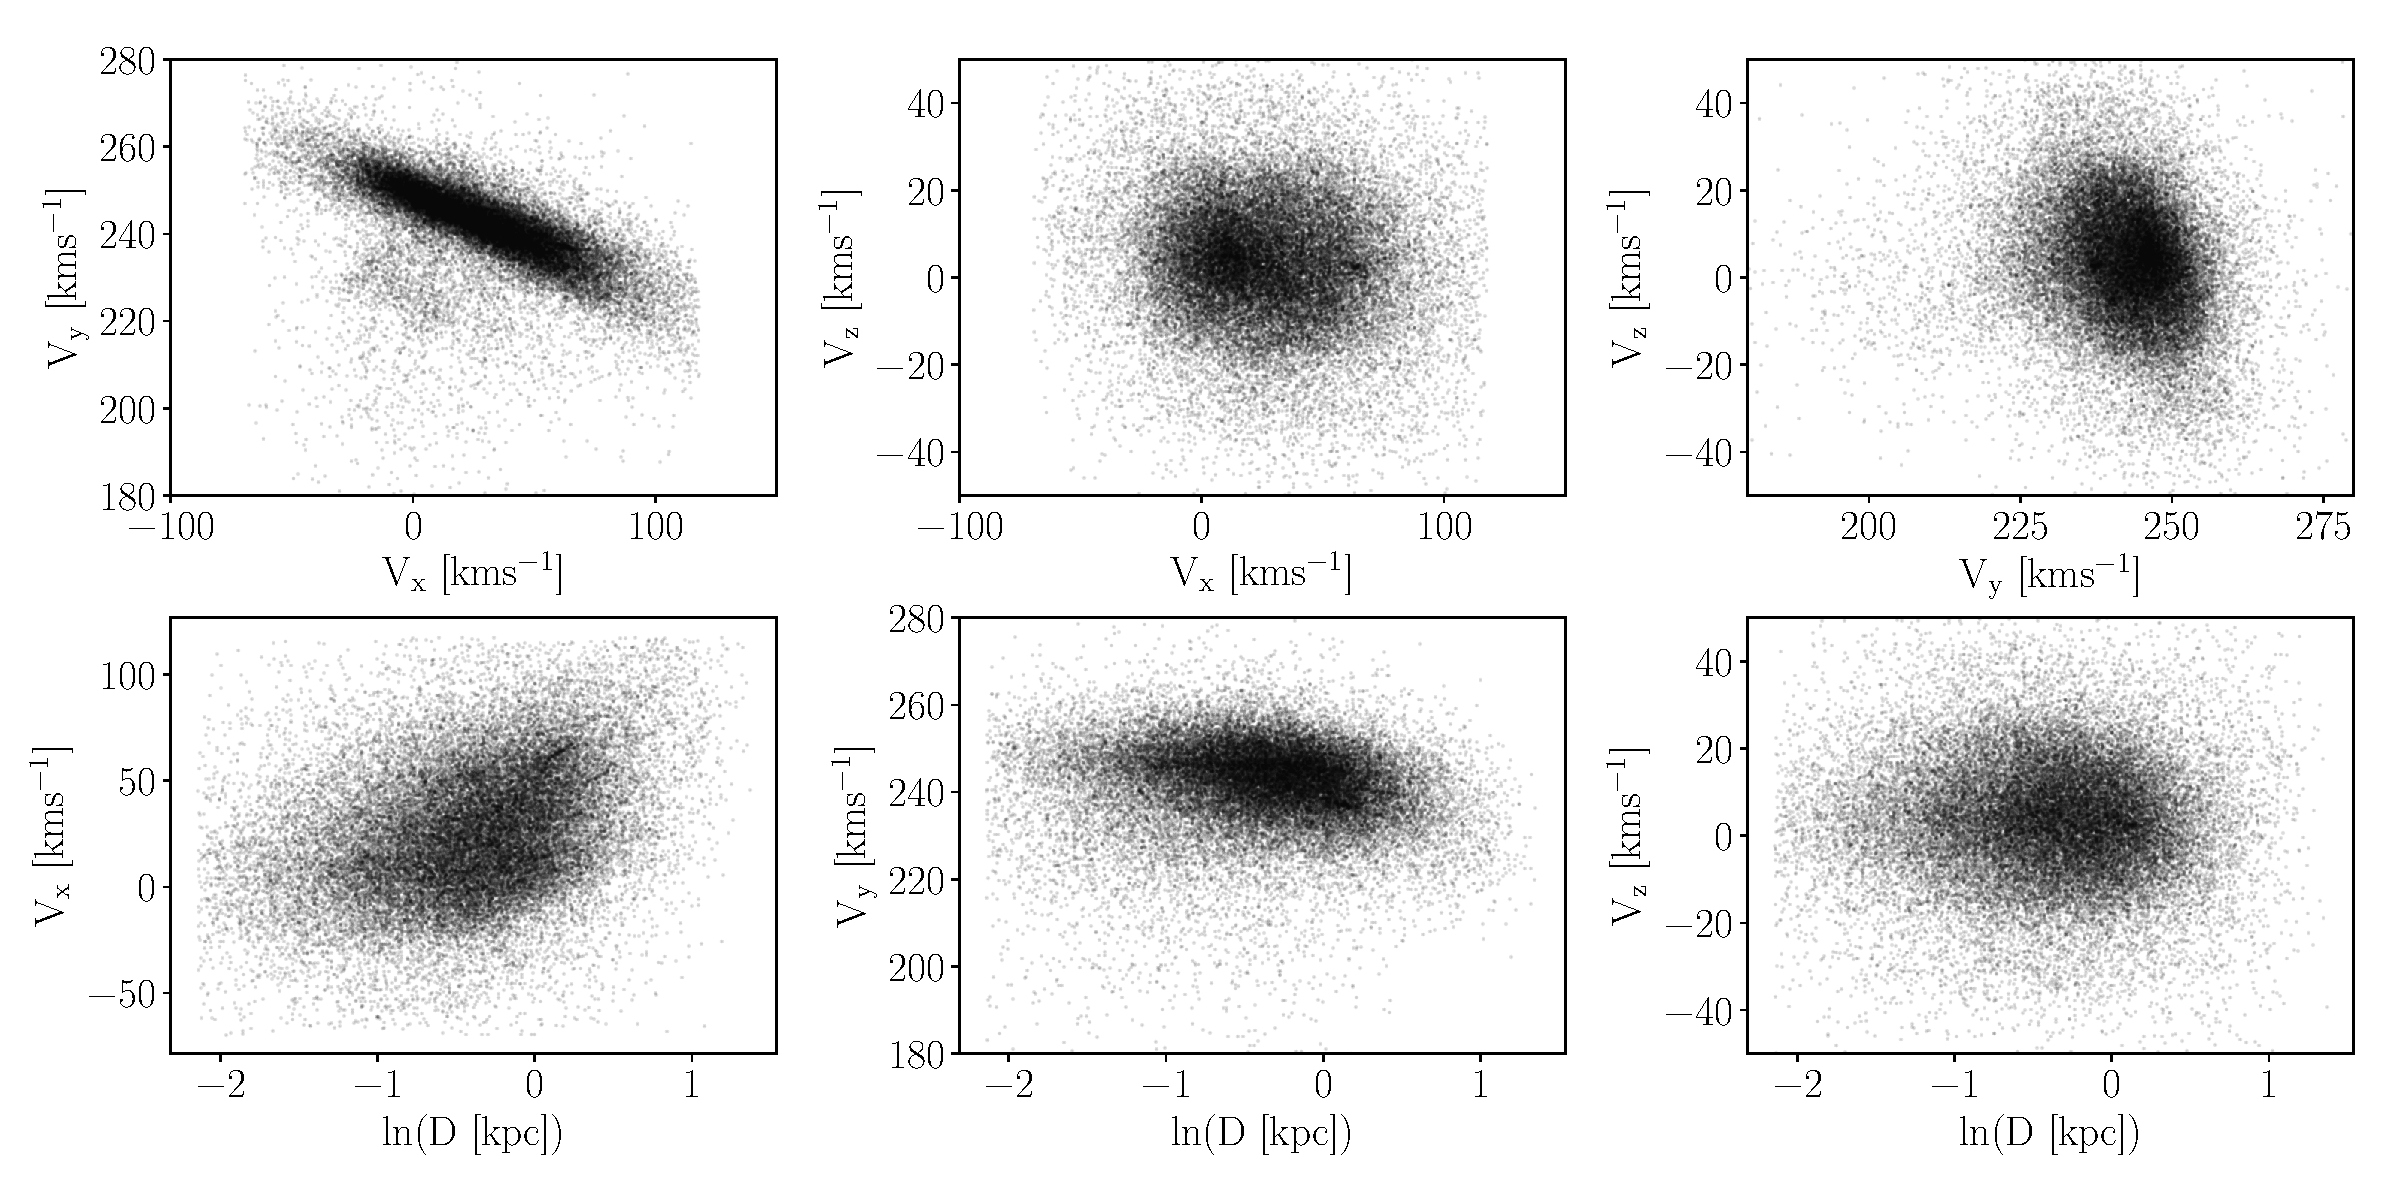
\includegraphics[width=1\textwidth]{prior_distributions}
\label{fig:prior_distributions}
\end{figure}

We tuned the {\it PyMC3} model for 1500 steps, with a target acceptance
fraction of 0.9.
The model was then run for 1000 steps with 4 chains.

Figure \ref{fig:v_comparison} shows the \vx, \vy\ and \vz\ velocities we
inferred, compared with those calculated from measured RVs.
2000 stars are shown, which were chosen at random from the \kepler\ rotators
with RV measurements.
\begin{figure}[ht!]
\caption{Vertical velocities calculated with full 6D information vs vertical
    velocities inferred without RV, for all 3000 \mct\ stars with \gaia\ RV
    measurements.}
  \centering
    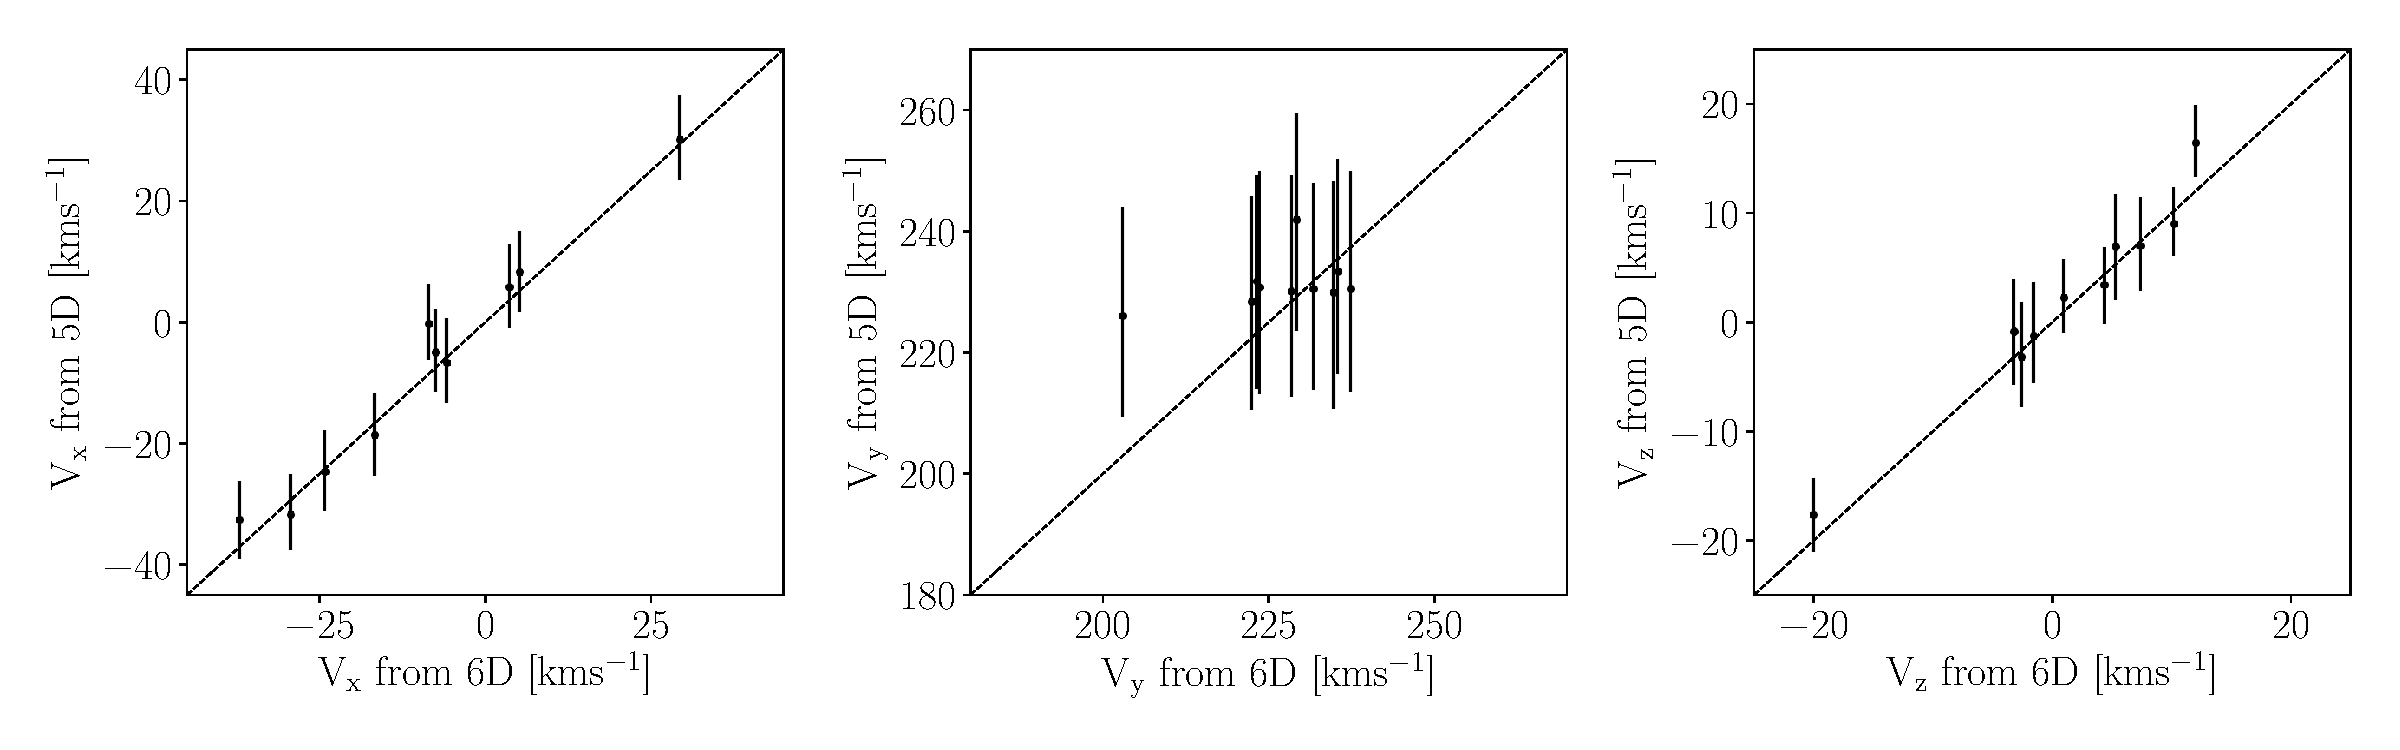
\includegraphics[width=1\textwidth]{v_comparison}
\label{fig:v_comparison}
\end{figure}
The \kepler\ field is oriented almost along the \y\-axis of the Galactocentric
coordinate system.
As a result, \x\ and \z-direction velocities of \kepler\ stars are extremely
well-constrained with proper motion alone, but \vy\ is almost completely
unconstrained without an RV.
Figure \ref{fig:v_comparison} shows that \vx\ and \vz\ velocities inferred
without RV measurements are extremely similar to those calculated with RVs.

\subsection{Calculating velocity dispersions}
\label{sec:velocity_dispersion}

A kinematic age can be calculated from the velocity dispersion, \ie\ standard
deviation, of a group of stars.
These velocity dispersions can then be converted into an age using an AVR
\citep[\eg][]{holmberg2009, yu2018}.
Kinematic ages represent the {\it average age} of a group of stars and are
most informative when stars are grouped by age.
If a group of stars have similar ages, their kinematic age will be close
the age of each individual.
On the other hand, the kinematic age of a group with large age variance will
not provide much information about the ages of individual stars.
Velocity distributions themselves do not reveal whether a group of stars have
similar or different ages, since either case the velocities are
Gaussian-distributed.
Fortunately however, we can group \kepler\ stars by age using the implicit
assumption that underpins gyrochronology: that stars with the same rotation
period and color are the same age.
We discuss the implications of this assumption and cases where it doesn't
apply in the Discussion of this paper (section \ref{sec:discussion}).

In this paper, we calculated the kinematic age of {\it each individual star}
in our sample, by grouping it with its neighbors in \logp--\teff\ space.
This method is similar to calculating a rolling, or running standard
deviation and allowed us to assign a unique age to each star.
However, ages calculated this way are tightly correlated, and their
correlation depends strongly on window-size.

% To calculate a \vz\ velocity dispersion and kinematic age for each \kepler\
% rotator, we grouped stars with their neighbors in \logp--\teff\ space.
We tested two methods of grouping stars: K-nearest neighbors, and bins in
\logp\ and \teff .
In the K-nearest neighbors method, each star was grouped with the K-nearest
stars in \logp-\teff\ space.
Groups created this way spanned a small \logp -\teff\ range where the stellar
number density was large, and a large range where the number density was
small.
In other words, the number of stars was fixed but the window-size changed.
In the fixed range method, stars were grouped within a fixed \logp -\teff
window.
This method created groups with large numbers of stars in densely populated
regions of the \logp--\teff\ plane, and small numbers of stars in sparsely
populated regions, \ie\ the number of stars changed but the window-size was
fixed.
To choose the best method, and to optimize for the parameters of each (K and
window-size), we conducted a set of tests.

\subsection{Converting velocity dispersion to age with an AVR}
\label{sec:avr}
We used the \citet{yu2018} AVR to convert velocity dispersion to age.
This relation was calibrated using the ages and velocities of red clump stars.
They divided their sample into metal rich and poor subsets, and calibrated
separate AVRs for each, plus a global AVR.
Their AVR is a power law:
\begin{equation}
    \sigma_{vz} = \alpha t ^\beta,
\end{equation}
where $\alpha$ and $\beta$ take values (6.38, 0.578) for metal rich stars
(3.89, 1.01) for metal poor stars, and (5.47, 0.765) for all stars.

We used 1.5$\times$ the Median Absolute Deviation (MAD) of velocities, which
is a robust approximation to the standard deviation and is less sensitive to
outliers.
Velocity outliers could be binary stars or could be generated by
underestimated parallax or proper motion uncertainties.

\subsection{Comparing kinematic ages with asteroseismic and cluster ages}

\subsection{A Gaussian process gyrochronology relation}
\label{sec:gp_model}
